\documentclass{article}
\usepackage[utf8]{inputenc}
\usepackage{graphicx}
\usepackage{tikz}
\usepackage{todonotes}
\usepackage{hyperref}
\usetikzlibrary{arrows, arrows.meta}
\usepackage{float}
\usepackage[]{algorithm2e}
\usepackage{pgfplots}

% Use standard A4 paper and standard margins for A4.
\usepackage[a4paper, margin=2.54cm]{geometry}

\begin{document}
\begin{titlepage}
    \begin{center}
       \vspace*{4cm}

       \textbf{\LARGE Tetris Project for AOS}

       \vspace{1.5cm}
        Design Document for the Tetris project for the course "Advanced Operating System".
            
       \vfill

       \textbf{Authors:}\\
       Accordi Gianmarco\\
       Chierici Franco

       \vspace{0.8cm}
     
       
\includegraphics[width=0.4\textwidth]{img/Logo_Politecnico_Milano.png}
            
       Dipartimento di Elettronica, Informazione e Bioingegneria\\
       Politecnico di Milano\\
       Italy\\
       29/03/2021
            
   \end{center}
\end{titlepage}

\tableofcontents

\newpage

\section{Introduction}
The scope of this document is to explain the design choice we have have made during the development of our project: a version of Tetris working from a terminal console, that is executed on an external microcontroller integrated circuit. 
It will also contains all the reference to better understand the structure of the code.

\section{Design and Interfaces}

\begin{figure}[H]
    \centering
    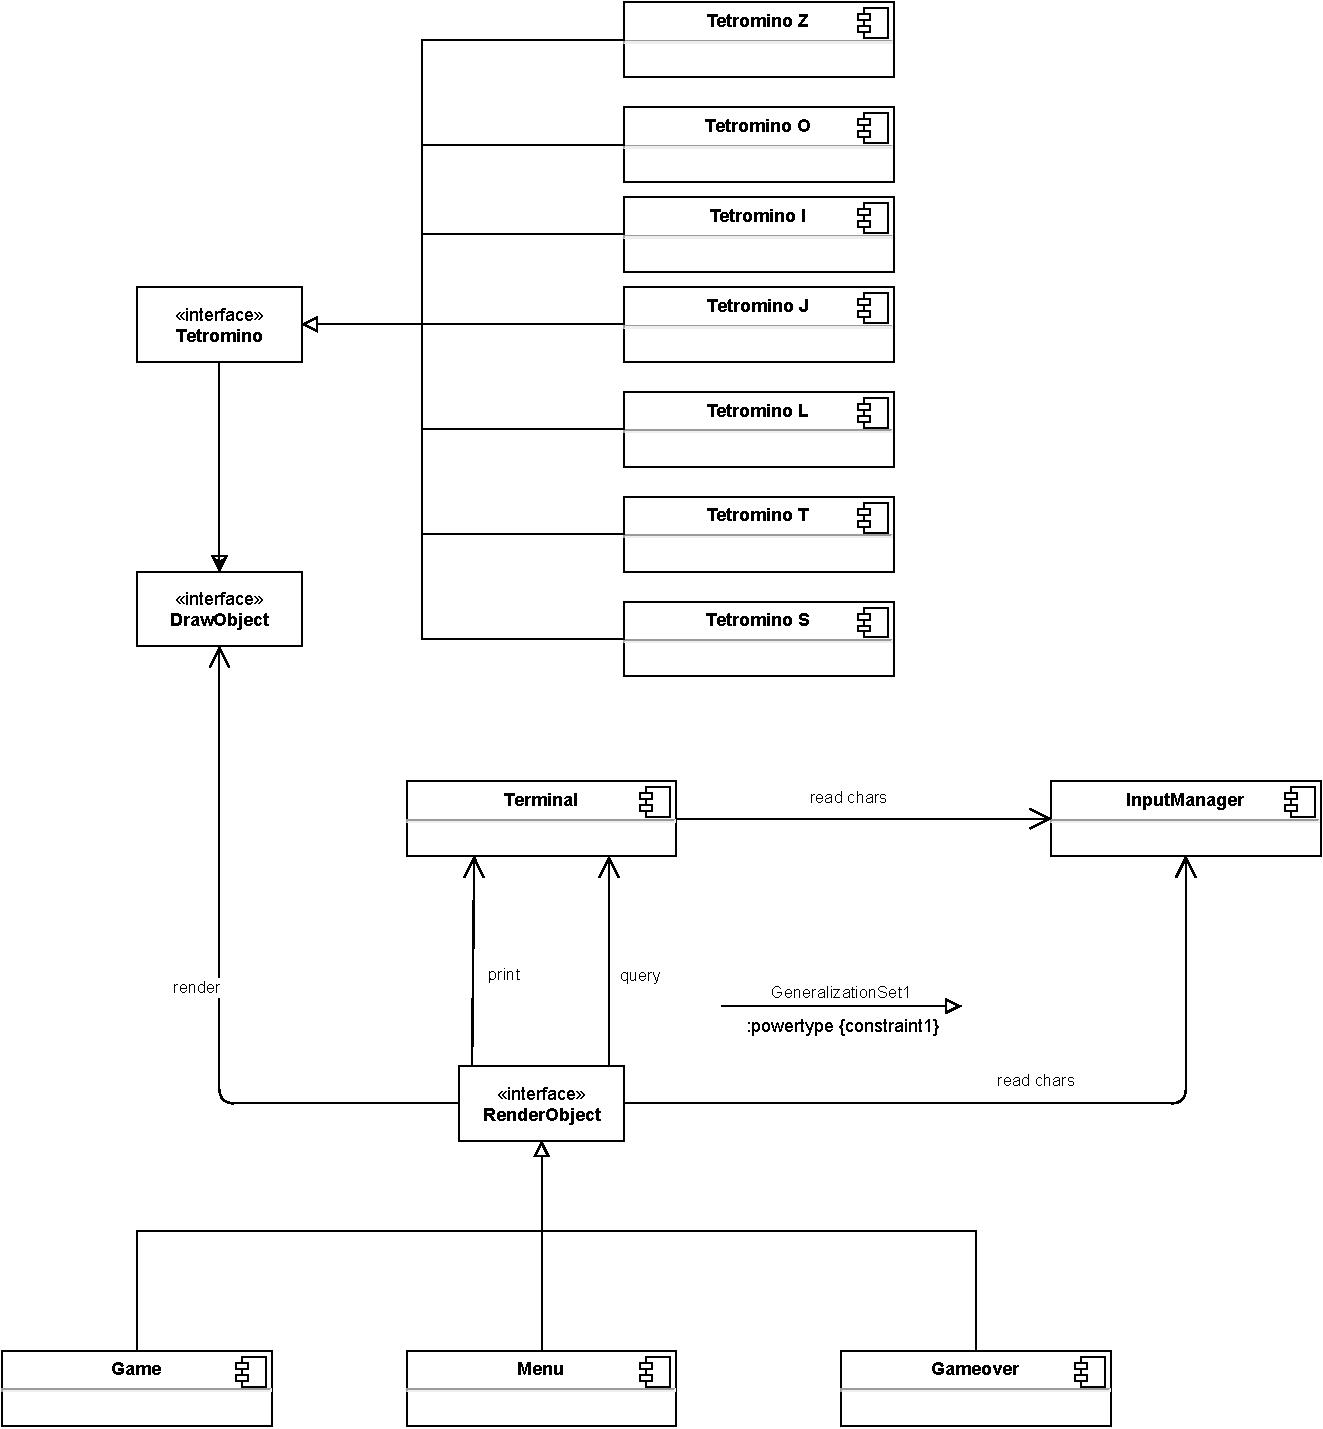
\includegraphics[width=\linewidth]{img/InterafcesDiagram.pdf}
    \caption{Interfaces Diagram of the project.}
    \label{fig:gather}
\end{figure}

\section{Target Platform}

\section{Implementation}
This part of the document better highlight what hwo we have proceed in the implementation of our project from a more technical perspective.

\subsection{Packages}
Our project has been developed by using C++\cite{slidec++}, in order to be compliant with the miosix-kernel\cite{miosix}.

\subsection{Terminal Rendering}


\subsection{Main Loop}
\begin{algorithm}[H]
    Setup of the InputManager and the Terminal\;
    \While{!isDone} {\
        Synchronized with MPI\_Barrier(MPI\_COMM\_WORLD)\;
        \eIf{myID==processorID}{
            Allocate enough buffer in order to receive from each processor information about the amount of data it will send\;      
        }
        {
            Prepare the information about the amount of data to be sent\;
        }
        Perform an MPI\_Gather\;       
        \eIf{myID==processorID}{
            Allocate enough buffer, based on the information received in the previous gather, in order to receive from each processor the data it will send\;    
        }
        {
            Prepare the data to be sent\;
        }
        Perform an MPI\_Gatherv\;
    }
    \caption{Main loop executed inside the main.cpp.}
\end{algorithm}

\subsection{Development Note}
In order to proceed with the development of our project, we have locally cloned the github repository of the miosix kernel\footnote{https://github.com/fedetft/miosix-kernel}.
After removing the \emph{.git} folder, we have also cloned into the same folder our repository\footnote{https://github.com/gianfi12/AOS-Tetris}.
In order to keep our code more parametric as possible we have defined an header file at \path{terminal/utility.h} that acts as a configuration file 

\section{Usage and Setup}


\bibliographystyle{plain}
\bibliography{references}
\end{document}